\documentclass[12pt]{article}
\usepackage[margin=2.5cm]{geometry}
\usepackage{enumerate}
\usepackage{amsfonts}
\usepackage{amsmath}
\usepackage{fancyhdr}
\usepackage{amsmath}
\usepackage{amssymb}
\usepackage{amsthm}
\usepackage{mdframed}
\usepackage{graphicx}
\usepackage{subcaption}
\usepackage{adjustbox}
\usepackage{listings}
\usepackage{xcolor}
\usepackage{booktabs}
\usepackage[utf]{kotex}
\usepackage{hyperref}

\definecolor{codegreen}{rgb}{0,0.6,0}
\definecolor{codegray}{rgb}{0.5,0.5,0.5}
\definecolor{codepurple}{rgb}{0.58,0,0.82}
\definecolor{backcolour}{rgb}{0.95,0.95,0.92}

\lstdefinestyle{mystyle}{
    backgroundcolor=\color{backcolour},
    commentstyle=\color{codegreen},
    keywordstyle=\color{magenta},
    numberstyle=\tiny\color{codegray},
    stringstyle=\color{codepurple},
    basicstyle=\ttfamily\footnotesize,
    breakatwhitespace=false,
    breaklines=true,
    captionpos=b,
    keepspaces=true,
    numbers=left,
    numbersep=5pt,
    showspaces=false,
    showstringspaces=false,
    showtabs=false,
    tabsize=1
}

\lstset{style=mystyle}

\pagestyle{fancy}
\renewcommand{\headrulewidth}{0.4pt}
\lhead{CSC 373}
\rhead{Worksheet 1 Solution}

\begin{document}
\title{CSC373 Worksheet 1 Solution}
\maketitle

\bigskip

\begin{enumerate}[1.]
    \item

    \bigskip

    \underline{\textbf{Notes:}}

    \begin{itemize}
        \item Strassen's method for matrix multiplication

        \begin{itemize}
            \item Reduces the time complexity of matrix multiplication from $O(n^3)$ to $O(n^{\log_2 7}) = O(n^{2.81})$

            \item Has four steps

            \bigskip

            \begin{enumerate}[1)]
                \item Divide the input matrics $A$ and $B$ and output matrix $C$
                into $n/2 \times n/2$ submatrices

                \begin{center}
                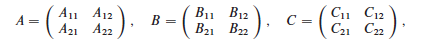
\includegraphics[width=0.7\linewidth]{images/worksheet_1_solution_1.png}
                \end{center}
            \end{enumerate}

            \item Is not preferred in practical purposes

            \bigskip

            \begin{enumerate}[1)]
                \item The constants used in Strassen’s method are high and for a typical application Naive method works better.
                \item For Sparse matrices, there are better methods especially designed for them.
                \item The submatrices in recursion take extra space.
                \item Because of the limited precision of computer arithmetic on noninteger values, larger errors accumulate in Strassen’s algorithm than in Naive Method
            \end{enumerate}
        \end{itemize}

        \bigskip

        \underline{\textbf{References:}}

        \bigskip

        \begin{enumerate}[1)]
            \item GeeksForGeeks, Divide and Conquer | Set 5 (Strassen’s Matrix Multiplication), \href{https://www.geeksforgeeks.org/strassens-matrix-multiplication/}{link}
        \end{enumerate}

        \item Regular matrix multiplication

        \begin{itemize}
            \item
        \end{itemize}
    \end{itemize}
\end{enumerate}

\end{document}